\section{Event Retransmission Response Packet Processing Module} 

The Event Retransmission Request Packet Processing module takes an
input event retransmit request and attempts to acquire that packet
from the retx Buffer interface. It then sends that packet out to the
interface. Note that the packet retrieved from the FIFO may not be the
packet requested, if the FIFO has since wrapped around.

\begin{figure}
\begin{centering}
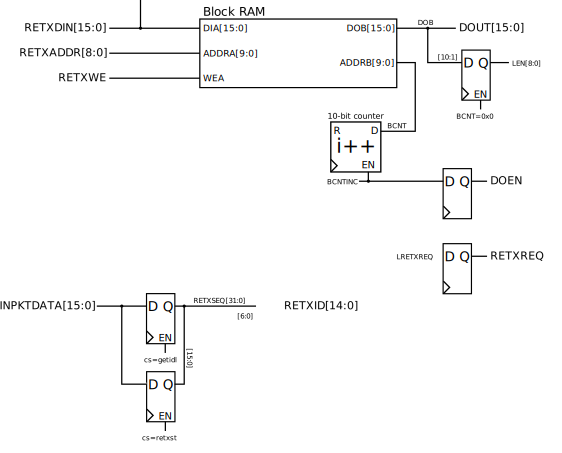
\includegraphics[scale=0.8]{eventretxresponse.svg}
\end{centering}
\caption{Retransmission Request module.}
\label{eventretxresponse}
\end{figure}

\begin{figure}
\begin{centering}
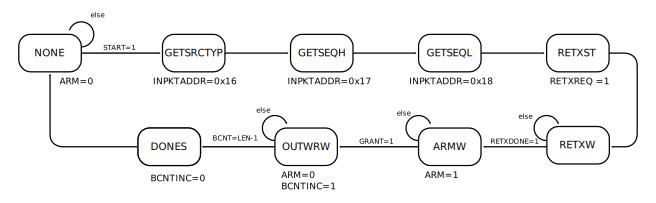
\includegraphics[scale=0.8]{eventretxresponse.fsm.svg}
\end{centering}
\caption{Event Retransmission Request module FSM.}
\label{eventretxresponse.fsm}
\end{figure}
